\documentclass{standalone}
\usepackage{tikz}
\usetikzlibrary{patterns, positioning}

\begin{document}
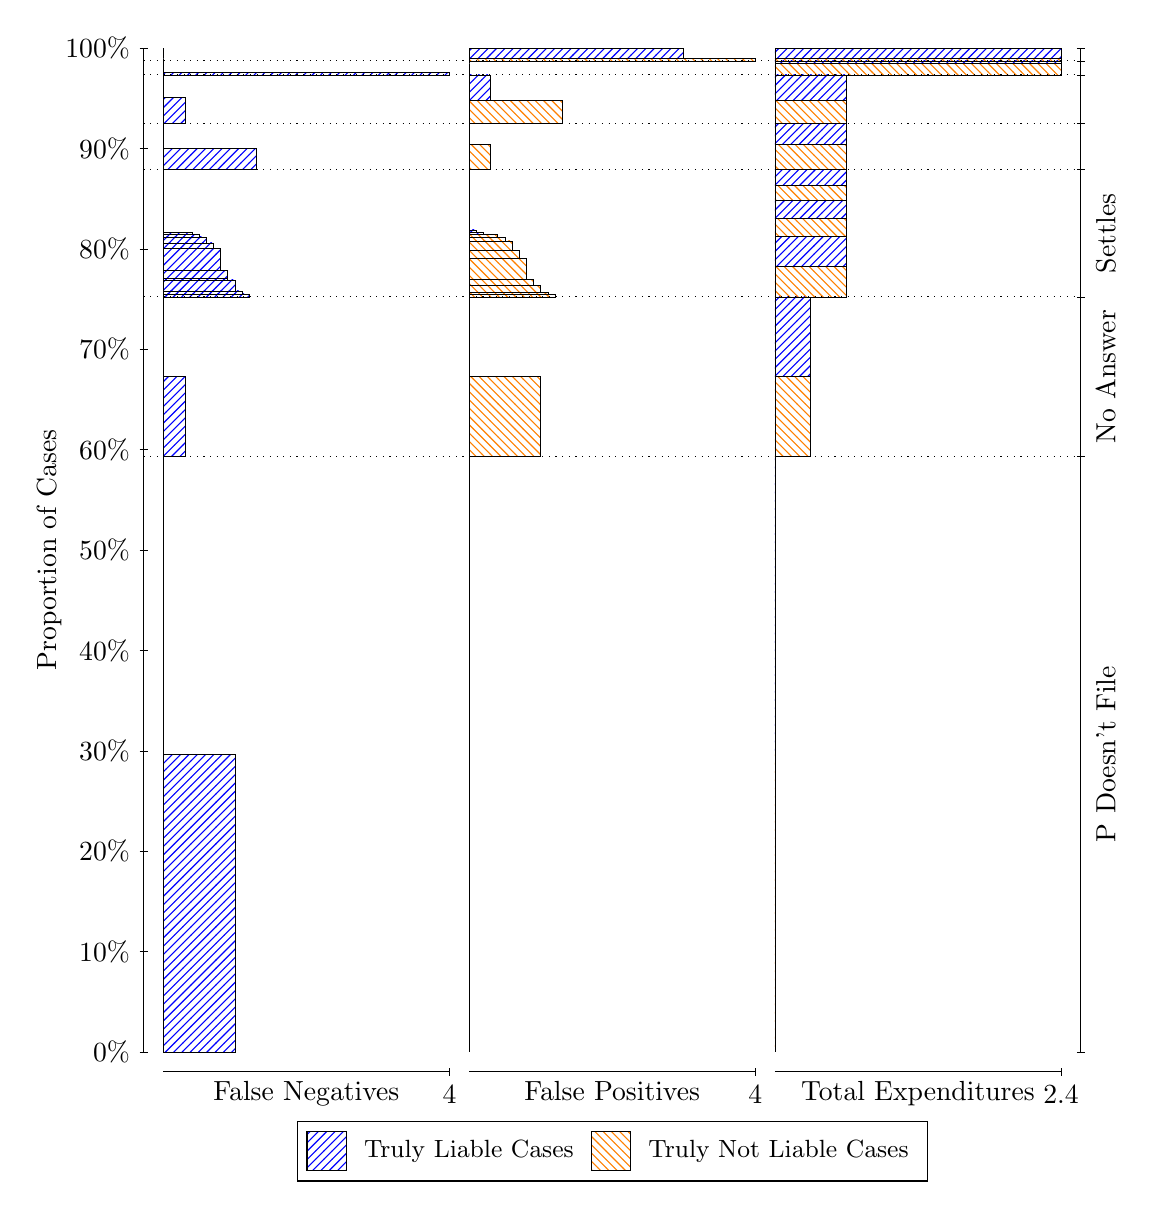
\begin{tikzpicture}
\draw[black, very thin] (1.5,1.75) -- (1.5,14.5);
\node[rotate=90, anchor=center] at (0.3, 8.125) {Proportion of Cases};
\draw[black, very thin] (1.45,1.75) -- (1.55,1.75);
\node[anchor=east] at (1.45, 1.75) {0\%};
\draw[black, very thin] (1.45,3.025) -- (1.55,3.025);
\node[anchor=east] at (1.45, 3.025) {10\%};
\draw[black, very thin] (1.45,4.3) -- (1.55,4.3);
\node[anchor=east] at (1.45, 4.3) {20\%};
\draw[black, very thin] (1.45,5.575) -- (1.55,5.575);
\node[anchor=east] at (1.45, 5.575) {30\%};
\draw[black, very thin] (1.45,6.85) -- (1.55,6.85);
\node[anchor=east] at (1.45, 6.85) {40\%};
\draw[black, very thin] (1.45,8.125) -- (1.55,8.125);
\node[anchor=east] at (1.45, 8.125) {50\%};
\draw[black, very thin] (1.45,9.4) -- (1.55,9.4);
\node[anchor=east] at (1.45, 9.4) {60\%};
\draw[black, very thin] (1.45,10.675) -- (1.55,10.675);
\node[anchor=east] at (1.45, 10.675) {70\%};
\draw[black, very thin] (1.45,11.95) -- (1.55,11.95);
\node[anchor=east] at (1.45, 11.95) {80\%};
\draw[black, very thin] (1.45,13.225) -- (1.55,13.225);
\node[anchor=east] at (1.45, 13.225) {90\%};
\draw[black, very thin] (1.45,14.5) -- (1.55,14.5);
\node[anchor=east] at (1.45, 14.5) {100\%};

\draw[black, very thin] (13.4,1.75) -- (13.4,14.5);
\draw[black, very thin] (13.35,1.75) -- (13.45,1.75);
\node[anchor=west] at (13.35, 1.75) {};
\draw[black, very thin] (13.35,9.3149) -- (13.45,9.3149);
\node[anchor=west] at (13.35, 9.3149) {};
\draw[black, very thin] (13.35,11.339) -- (13.45,11.339);
\node[anchor=west] at (13.35, 11.339) {};
\draw[black, very thin] (13.35,12.954) -- (13.45,12.954);
\node[anchor=west] at (13.35, 12.954) {};
\draw[black, very thin] (13.35,13.545) -- (13.45,13.545);
\node[anchor=west] at (13.35, 13.545) {};
\draw[black, very thin] (13.35,14.16) -- (13.45,14.16);
\node[anchor=west] at (13.35, 14.16) {};
\draw[black, very thin] (13.35,14.337) -- (13.45,14.337);
\node[anchor=west] at (13.35, 14.337) {};
\draw[black, very thin] (13.35,14.5) -- (13.45,14.5);
\node[anchor=west] at (13.35, 14.5) {};

\draw[black, very thin, pattern color=blue, pattern=north east lines] (1.75,1.75) rectangle (2.6583,5.5324);
\draw[black, very thin, pattern color=orange, pattern=north west lines] (1.75,5.5324) rectangle (1.75,9.3149);
\draw[black, very thin, pattern color=blue, pattern=north east lines] (1.75,9.3149) rectangle (2.0225,10.327);
\draw[black, very thin, pattern color=orange, pattern=north west lines] (1.75,10.327) rectangle (1.75,11.339);
\draw[black, very thin, pattern color=blue, pattern=north east lines] (1.75,11.339) rectangle (2.84,11.377);
\draw[black, very thin, pattern color=blue, pattern=north east lines] (1.75,11.377) rectangle (2.7492,11.416);
\draw[black, very thin, pattern color=blue, pattern=north east lines] (1.75,11.416) rectangle (2.6583,11.555);
\draw[black, very thin, pattern color=blue, pattern=north east lines] (1.75,11.555) rectangle (2.5675,11.575);
\draw[black, very thin, pattern color=blue, pattern=north east lines] (1.75,11.575) rectangle (2.5675,11.676);
\draw[black, very thin, pattern color=blue, pattern=north east lines] (1.75,11.676) rectangle (2.4767,11.959);
\draw[black, very thin, pattern color=blue, pattern=north east lines] (1.75,11.959) rectangle (2.3858,12.026);
\draw[black, very thin, pattern color=blue, pattern=north east lines] (1.75,12.026) rectangle (2.295,12.102);
\draw[black, very thin, pattern color=blue, pattern=north east lines] (1.75,12.102) rectangle (2.2042,12.131);
\draw[black, very thin, pattern color=blue, pattern=north east lines] (1.75,12.131) rectangle (2.1133,12.159);
\draw[black, very thin, pattern color=orange, pattern=north west lines] (1.75,12.159) rectangle (1.75,12.954);
\draw[black, very thin, pattern color=blue, pattern=north east lines] (1.75,12.954) rectangle (2.9308,13.226);
\draw[black, very thin, pattern color=orange, pattern=north west lines] (1.75,13.226) rectangle (1.75,13.545);
\draw[black, very thin, pattern color=blue, pattern=north east lines] (1.75,13.545) rectangle (2.0225,13.871);
\draw[black, very thin, pattern color=orange, pattern=north west lines] (1.75,13.871) rectangle (1.75,14.16);
\draw[black, very thin, pattern color=blue, pattern=north east lines] (1.75,14.16) rectangle (5.3833,14.192);
\draw[black, very thin, pattern color=orange, pattern=north west lines] (1.75,14.192) rectangle (1.75,14.337);
\draw[black, very thin, pattern color=orange, pattern=north west lines] (1.75,14.337) rectangle (1.75,14.369);
\draw[black, very thin, pattern color=blue, pattern=north east lines] (1.75,14.369) rectangle (1.75,14.5);
\draw[black, very thin, pattern color=orange, pattern=north west lines] (5.6333,1.75) rectangle (5.6333,5.5325);
\draw[black, very thin, pattern color=blue, pattern=north east lines] (5.6333,5.5325) rectangle (5.6333,9.3149);
\draw[black, very thin, pattern color=orange, pattern=north west lines] (5.6333,9.3149) rectangle (6.5417,10.327);
\draw[black, very thin, pattern color=blue, pattern=north east lines] (5.6333,10.327) rectangle (5.6333,11.339);
\draw[black, very thin, pattern color=orange, pattern=north west lines] (5.6333,11.339) rectangle (6.7233,11.369);
\draw[black, very thin, pattern color=orange, pattern=north west lines] (5.6333,11.369) rectangle (6.6325,11.399);
\draw[black, very thin, pattern color=orange, pattern=north west lines] (5.6333,11.399) rectangle (6.5417,11.485);
\draw[black, very thin, pattern color=orange, pattern=north west lines] (5.6333,11.485) rectangle (6.4508,11.562);
\draw[black, very thin, pattern color=orange, pattern=north west lines] (5.6333,11.562) rectangle (6.36,11.828);
\draw[black, very thin, pattern color=orange, pattern=north west lines] (5.6333,11.828) rectangle (6.2692,11.931);
\draw[black, very thin, pattern color=orange, pattern=north west lines] (5.6333,11.931) rectangle (6.1783,12.052);
\draw[black, very thin, pattern color=orange, pattern=north west lines] (5.6333,12.052) rectangle (6.0875,12.091);
\draw[black, very thin, pattern color=orange, pattern=north west lines] (5.6333,12.091) rectangle (5.9967,12.134);
\draw[black, very thin, pattern color=blue, pattern=north east lines] (5.6333,12.134) rectangle (5.815,12.162);
\draw[black, very thin, pattern color=blue, pattern=north east lines] (5.6333,12.162) rectangle (5.7242,12.191);
\draw[black, very thin, pattern color=blue, pattern=north east lines] (5.6333,12.191) rectangle (5.6333,12.954);
\draw[black, very thin, pattern color=orange, pattern=north west lines] (5.6333,12.954) rectangle (5.9058,13.273);
\draw[black, very thin, pattern color=blue, pattern=north east lines] (5.6333,13.273) rectangle (5.6333,13.545);
\draw[black, very thin, pattern color=orange, pattern=north west lines] (5.6333,13.545) rectangle (6.8142,13.834);
\draw[black, very thin, pattern color=blue, pattern=north east lines] (5.6333,13.834) rectangle (5.9058,14.16);
\draw[black, very thin, pattern color=orange, pattern=north west lines] (5.6333,14.16) rectangle (5.6333,14.304);
\draw[black, very thin, pattern color=blue, pattern=north east lines] (5.6333,14.304) rectangle (5.6333,14.337);
\draw[black, very thin, pattern color=orange, pattern=north west lines] (5.6333,14.337) rectangle (9.2667,14.369);
\draw[black, very thin, pattern color=blue, pattern=north east lines] (5.6333,14.369) rectangle (8.3583,14.5);
\draw[black, very thin, pattern color=orange, pattern=north west lines] (9.5167,1.75) rectangle (9.5167,5.5325);
\draw[black, very thin, pattern color=blue, pattern=north east lines] (9.5167,5.5325) rectangle (9.5167,9.3149);
\draw[black, very thin, pattern color=orange, pattern=north west lines] (9.5167,9.3149) rectangle (9.9708,10.327);
\draw[black, very thin, pattern color=blue, pattern=north east lines] (9.5167,10.327) rectangle (9.9708,11.339);
\draw[black, very thin, pattern color=orange, pattern=north west lines] (9.5167,11.339) rectangle (10.425,11.722);
\draw[black, very thin, pattern color=blue, pattern=north east lines] (9.5167,11.722) rectangle (10.425,12.109);
\draw[black, very thin, pattern color=orange, pattern=north west lines] (9.5167,12.109) rectangle (10.425,12.332);
\draw[black, very thin, pattern color=blue, pattern=north east lines] (9.5167,12.332) rectangle (10.425,12.568);
\draw[black, very thin, pattern color=orange, pattern=north west lines] (9.5167,12.568) rectangle (10.425,12.757);
\draw[black, very thin, pattern color=blue, pattern=north east lines] (9.5167,12.757) rectangle (10.425,12.954);
\draw[black, very thin, pattern color=orange, pattern=north west lines] (9.5167,12.954) rectangle (10.425,13.273);
\draw[black, very thin, pattern color=blue, pattern=north east lines] (9.5167,13.273) rectangle (10.425,13.545);
\draw[black, very thin, pattern color=orange, pattern=north west lines] (9.5167,13.545) rectangle (10.425,13.834);
\draw[black, very thin, pattern color=blue, pattern=north east lines] (9.5167,13.834) rectangle (10.425,14.16);
\draw[black, very thin, pattern color=orange, pattern=north west lines] (9.5167,14.16) rectangle (13.15,14.304);
\draw[black, very thin, pattern color=blue, pattern=north east lines] (9.5167,14.304) rectangle (13.15,14.337);
\draw[black, very thin, pattern color=orange, pattern=north west lines] (9.5167,14.337) rectangle (13.15,14.369);
\draw[black, very thin, pattern color=blue, pattern=north east lines] (9.5167,14.369) rectangle (13.15,14.5);
\draw[black, dotted] (1.5,9.3149) -- (13.4,9.3149);
\draw[black, dotted] (1.5,11.339) -- (13.4,11.339);
\draw[black, dotted] (1.5,12.954) -- (13.4,12.954);
\draw[black, dotted] (1.5,13.545) -- (13.4,13.545);
\draw[black, dotted] (1.5,14.16) -- (13.4,14.16);
\draw[black, dotted] (1.5,14.337) -- (13.4,14.337);
\draw[black, very thin] (1.75,1.5) -- (5.3833,1.5);
\node[anchor=north] at (3.5667, 1.5) {False Negatives};
\draw[black, very thin] (5.3833,1.45) -- (5.3833,1.55);
\node[anchor=north] at (5.3833, 1.45) {4};

\draw[black, very thin] (5.6333,1.5) -- (9.2667,1.5);
\node[anchor=north] at (7.45, 1.5) {False Positives};
\draw[black, very thin] (9.2667,1.45) -- (9.2667,1.55);
\node[anchor=north] at (9.2667, 1.45) {4};

\draw[black, very thin] (9.5167,1.5) -- (13.15,1.5);
\node[anchor=north] at (11.333, 1.5) {Total Expenditures};
\draw[black, very thin] (13.15,1.45) -- (13.15,1.55);
\node[anchor=north] at (13.15, 1.45) {2.4};

\node[black, centered, rotate=90] at (13.72, 5.5325) {P Doesn't File};
\node[black, centered, rotate=90] at (13.72, 10.327) {No Answer};
\node[black, centered, rotate=90] at (13.72, 12.147) {Settles};





\draw (7.449999999999999,1.5) node[draw=none] (baseCoordinate) {};
\begin{scope}[align=center]
        \matrix[scale=0.5, draw=black, below=0.5cm of baseCoordinate, nodes={draw}, column sep=0.1cm]{
            \node[rectangle, draw, minimum width=0.5cm, minimum height=0.5cm, pattern=north east lines, pattern color=blue] {}; &
            \node[draw=none, font=\small] (B) {Truly Liable Cases}; &
            \node[rectangle, draw, minimum width=0.5cm, minimum height=0.5cm, pattern=north west lines, pattern color=orange] {}; &
            \node[draw=none, font=\small] (B) {Truly Not Liable Cases}; \\
            };
\end{scope}

\end{tikzpicture}
\end{document}